\documentclass[letterpaper]{article}
\usepackage{format/aaai}
\usepackage{times}
\usepackage{helvet} % ZG
\usepackage{courier} % ZG
\frenchspacing
\setlength{\pdfpagewidth}{8.5in}
\setlength{\pdfpageheight}{11in}
\pdfinfo{
/Title (Insert Your Title Here)
/Author (Put All Your Authors Here, Separated by Commas)}
\setcounter{secnumdepth}{0}  



% use Times
%\usepackage{times}
% For figures
\usepackage{graphicx} % more modern
%\usepackage{epsfig} % less modern
\usepackage{subfigure} 

% For citations
%\usepackage{natbib}

% For algorithms
%\usepackage{algorithm}
%\usepackage{algorithmic}
%\usepackage{algorithmicx}

% As of 2011, we use the hyperref package to produce hyperlinks in the
% resulting PDF.  If this breaks your system, please commend out the
% following usepackage line and replace \usepackage{icml2014} with
% \usepackage[nohyperref]{icml2014} above.
%\usepackage{hyperref}

% Packages hyperref and algorithmic misbehave sometimes.  We can fix
% this with the following command.
\usepackage{algorithm}
\usepackage{algorithmic}
\newcommand{\theHalgorithm}{\arabic{algorithm}}

% Employ the following version of the ``usepackage'' statement for
% submitting the draft version of the paper for review.  This will set
% the note in the first column to ``Under review.  Do not distribute.''
%\usepackage{format/icml2014} 
% Employ this version of the ``usepackage'' statement after the paper has
% been accepted, when creating the final version.  This will set the
% note in the first column to ``Proceedings of the...''
%\usepackage[accepted]{icml2014}

%\usepackage{times}
\usepackage{hyperref}
\usepackage{url}
\usepackage{color}
\usepackage{preamble}
\definecolor{mydarkblue}{rgb}{0,0.08,0.45}
\hypersetup{ %
    pdftitle={},
    pdfauthor={},
    pdfsubject={},
    pdfkeywords={},
    pdfborder=0 0 0,
    pdfpagemode=UseNone,
    colorlinks=true,
    linkcolor=mydarkblue,
    citecolor=mydarkblue,
    filecolor=mydarkblue,
    urlcolor=mydarkblue,
    pdfview=FitH}
    
    
\usepackage{amsmath, amsfonts, bm, lipsum, capt-of}
\usepackage{natbib, xcolor, wrapfig, booktabs, multirow, caption}
%\DeclareCaptionType{copyrightbox}
\usepackage{float}
\usepackage{datetime}

%\renewcommand{\baselinestretch}{0.99}

\def\ie{i.e.\ }
\def\eg{e.g.\ }
\def\etc{etc.\ }
\let\oldemptyset\emptyset
\let\emptyset 0

\newcommand{\procedurename}{ABCD}
\newcommand{\genText}[1]{{\sf #1}}

%\author{
%James Robert Lloyd\\
%University of Cambridge\\
%Department of Engineering\\
%\texttt{jrl44@cam.ac.uk}
%\And
%David Duvenaud\\
%University of Cambridge \\
%Department of Engineering \\
%\texttt{dkd23@cam.ac.uk}
%\And
%Roger Grosse\\
%M.I.T.\\
%Brain and Cognitive Sciences \\
%\texttt{rgrosse@mit.edu}
%\And
%Joshua B. Tenenbaum\\
%M.I.T.\\
%Brain and Cognitive Sciences \\
%\texttt{jbt@mit.edu}
%\And
%Zoubin Ghahramani\\
%University of Cambridge \\
%Department of Engineering \\
%\texttt{zoubin@eng.cam.ac.uk}
%}

\newcommand{\fix}{\marginpar{FIX}}
\newcommand{\new}{\marginpar{NEW}}

\setlength{\marginparwidth}{0.6in}
%%%%%%%%%%%%%%%%%%%%%%%%%%%%%%%%%%%%%%%%%%%%%%%%%%%%%%%%%%
%%%% EDITING HELPER FUNCTIONS  %%%%%%%%%%%%%%%%%%%%%%%%%%%
%%%%%%%%%%%%%%%%%%%%%%%%%%%%%%%%%%%%%%%%%%%%%%%%%%%%%%%%%%

%% NA: needs attention (rough writing whose correctness needs to be verified)
%% TBD: instructions for how to fix a gap ("Describe the propagation by ...")
%% PROBLEM: bug or missing crucial bit 

%% use \fXXX versions of these macros to put additional explanation into a footnote.  
%% The idea is that we don't want to interrupt the flow of the paper or make it 
%% impossible to read because there are a bunch of comments.

%% NA's (and TBDs, those less crucially) should be written so 
%% that they flow with the text.

\definecolor{WowColor}{rgb}{.75,0,.75}
\definecolor{SubtleColor}{rgb}{0,0,.50}

% inline
\newcommand{\NA}[1]{\textcolor{SubtleColor}{ {\tiny \bf ($\star$)} #1}}
\newcommand{\LATER}[1]{\textcolor{SubtleColor}{ {\tiny \bf ($\dagger$)} #1}}
\newcommand{\TBD}[1]{\textcolor{SubtleColor}{ {\tiny \bf (!)} #1}}
\newcommand{\PROBLEM}[1]{\textcolor{WowColor}{ {\bf (!!)} {\bf #1}}}

% as margin notes

\newcounter{margincounter}
\newcommand{\displaycounter}{{\arabic{margincounter}}}
\newcommand{\incdisplaycounter}{{\stepcounter{margincounter}\arabic{margincounter}}}

\newcommand{\fTBD}[1]{\textcolor{SubtleColor}{$\,^{(\incdisplaycounter)}$}\marginpar{\tiny\textcolor{SubtleColor}{ {\tiny $(\displaycounter)$} #1}}}

\newcommand{\fPROBLEM}[1]{\textcolor{WowColor}{$\,^{((\incdisplaycounter))}$}\marginpar{\tiny\textcolor{WowColor}{ {\bf $\mathbf{((\displaycounter))}$} {\bf #1}}}}

\newcommand{\fLATER}[1]{\textcolor{SubtleColor}{$\,^{(\incdisplaycounter\dagger)}$}\marginpar{\tiny\textcolor{SubtleColor}{ {\tiny $(\displaycounter\dagger)$} #1}}}


%% For submission, make all render blank.
%\renewcommand{\LATER}[1]{}
%\renewcommand{\fLATER}[1]{}
%\renewcommand{\TBD}[1]{}
%\renewcommand{\fTBD}[1]{}
%\renewcommand{\PROBLEM}[1]{}
%\renewcommand{\fPROBLEM}[1]{}
%\renewcommand{\NA}[1]{#1}  % Note, NA's pass through!


% The \icmltitle you define below is probably too long as a header.
% Therefore, a short form for the running title is supplied here:
%\icmltitlerunning{Automatic construction and natural-language description of nonparametric regression models}

\setcounter{secnumdepth}{2}

 \begin{document}
% The file aaai.sty is the style file for AAAI Press 
% proceedings, working notes, and technical reports.
%
\title{Automatic Construction and Natural-Language Description \\ of Nonparametric Regression Models}
\author{}
\maketitle


%\twocolumn[
%\icmltitle{Automatic Construction and Natural-language Description \\ of Nonparametric Regression Models
%}

% It is OKAY to include author information, even for blind
% submissions: the style file will automatically remove it for you
% unless you've provided the [accepted] option to the icml2014
% package.
%\icmlauthor{Your Name}{email@yourdomain.edu}
%\icmladdress{Your Fantastic Institute,
%            314159 Pi St., Palo Alto, CA 94306 USA}
%\icmlauthor{Your CoAuthor's Name}{email@coauthordomain.edu}
%\icmladdress{Their Fantastic Institute,
%            27182 Exp St., Toronto, ON M6H 2T1 CANADA}

% You may provide any keywords that you 
% find helpful for describing your paper; these are used to populate 
% the "keywords" metadata in the PDF but will not be shown in the document
%\icmlkeywords{}

%\vskip 0.3in
%]

\begin{abstract} 
This paper presents the beginnings of an automatic statistician, focusing on regression problems.
Our system explores an open-ended space of possible statistical models to discover a good explanation of the data, and then produces a detailed report with figures and natural-language text.

Our approach treats unknown functions nonparametrically using Gaussian processes, which has two important consequences.
First, Gaussian processes model functions in terms of high-level properties (e.g.\ smoothness, trends, periodicity,
changepoints).
Taken together with the compositional structure of our language of models, this allows us to automatically describe functions through a decomposition into additive parts.
Second, the use of flexible nonparametric models and a rich
language for composing them in an open-ended manner also results
in state-of-the-art extrapolation performance evaluated over 13 real time
series data sets from various domains.

\end{abstract} 

\allowdisplaybreaks

\section{Introduction}

Automating the process of statistical modeling would have a tremendous impact on fields that currently rely on expert statisticians, machine learning researchers, and data scientists.
While fitting simple models (such as linear regression) is largely automated by standard software packages, there has been little work on the automatic construction of flexible but interpretable models. 
What are the ingredients required for an artificial intelligence system to be able to perform statistical modeling automatically? 
In this paper we conjecture that the following ingredients may be useful for building an AI system for statistics, and we develop a working system which incorporates them:
\begin{itemize}
\item {\bf An open-ended language of models} expressive enough to
  capture many of the modeling assumptions and model composition
  techniques  applied by human statisticians to capture real-world phenomena
\item {\bf A search procedure} to efficiently explore the space of
  models spanned by the language
\item {\bf A principled method for evaluating models} in terms of their complexity and their degree of fit to the
  data
\item {\bf A procedure for automatically generating reports} which
  explain and visualize different factors underlying the data, make
  the chosen modeling assumptions explicit, and quantify how each
  component improves the predictive power of the model 
\end{itemize}

\begin{figure}[t]
\centering
\fbox{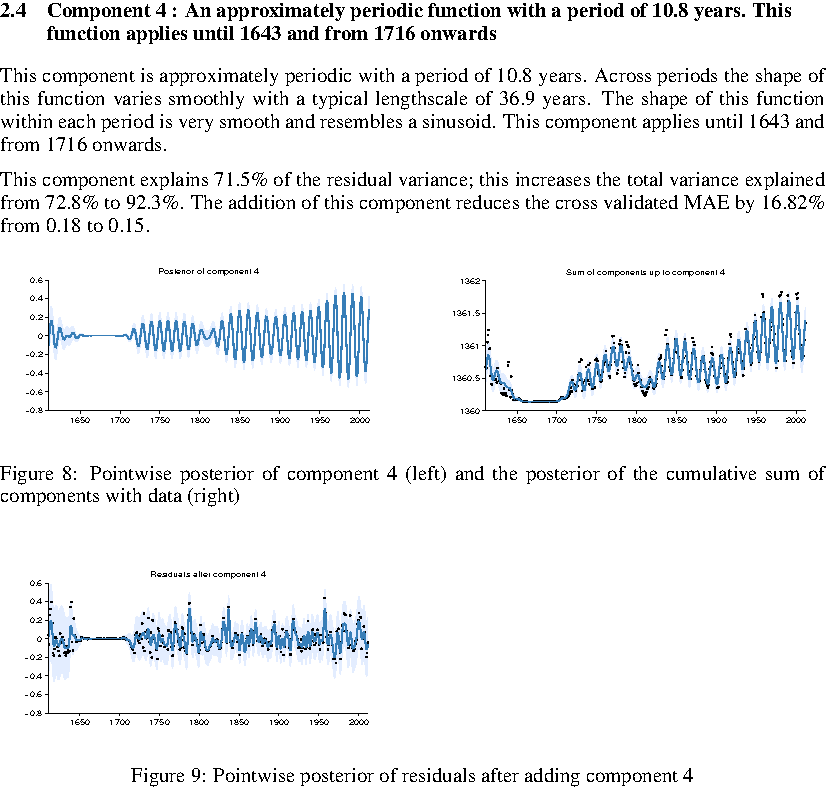
\includegraphics[trim=0cm 4.75cm 0cm 1.0cm, clip, width=0.98\columnwidth]{solarpages/pg_0007-crop}}
\caption{Extract from an automatically-generated report describing the model components discovered by automatic model search.  This part of the report isolates and describes the approximately 11-year sunspot cycle, also noting its disappearance during the 16th century, a time known as the Maunder minimum \citep{lean1995reconstruction}.}
\label{fig:periodic}
\end{figure}

In this paper,  we introduce a system for modeling time-series data
 containing the above ingredients which we call the Automatic
Bayesian Covariance Discovery (ABCD) system. The system defines an open-ended
language of Gaussian process models via a compositional grammar. The
space is searched greedily, using marginal likelihood and
the Bayesian Information Criterion (BIC) to evaluate models. The 
compositional structure of the language allows us to develop a method
for automatically translating components of the model into
natural-language descriptions of patterns in the data.

We show examples of automatically generated reports which highlight
interpretable features discovered in a variety of data sets (e.g.\
figure~\ref{fig:periodic}).  The supplementary material to this paper
includes 13 complete reports automatically generated by ABCD.

Good statistical modeling requires not only
interpretability but predictive accuracy. We compare ABCD against
existing model construction techniques in terms of predictive
performance at extrapolation, and we find state-of-the-art performance
on the 13 time series. In the remainder of this paper we describe the
components of ABCD in detail. 

\section{A language of regression models}
\label{sec:improvements}

% what is regression
The general problem of regression consists of learning a function $f$
mapping from some input space $\mathcal{X}$ to some output space
$\mathcal{Y}$. We would like an expressive language which can
represent both simple parametric forms of $f$ such as linear, polynomial, \etc and also complex nonparametric functions
specified in terms of properties such as smoothness, periodicity, \etc~
Fortunately, Gaussian processes (\gp{}s) provide a very general
and analytically tractable way of capturing both simple and complex
functions. 



% what is a GP /  kernel
Gaussian processes are distributions over functions such that any
finite subset of function evaluations, $(f(x_1), f(x_2), \ldots
f(x_N))$, have a joint Gaussian distribution
\citep{rasmussen38gaussian}. A \gp{} is completely specified by its
mean function, $\mu(x)=\mathbb{E}(f(x))$ and kernel (or covariance) function
$\kernel(x,x') = \Cov(f(x),f(x'))$.
It is common practice to assume zero mean,
since marginalizing over an unknown mean function can be equivalently
expressed as a zero-mean \gp{} with a new kernel. The structure of the
kernel captures high-level properties of the unknown function, $f$,
which in turn determines how the model generalizes or extrapolates to
new data.  We can therefore define a language of regression models by
specifying a language of kernels.

% kernels can be composed
The elements of this language are a set of  base
kernels capturing different function properties, and a set of
composition rules which combine kernels to yield other valid kernels.
Our base kernels are white noise ($\kWN$), constant ($\kC$), linear ($\kLin$), squared exponential ($\kSE$) and periodic ($\kPer$), which on their own encode for uncorrelated noise, constant functions, linear functions, smooth functions and periodic functions respectively\footnote{Definitions of kernels are in the supplementary material.}.
The composition rules are addition and multiplication:
%Addition and multiplication are defined as pointwise addition and multiplication of kernel functions:
\begin{align}
k_1 + k_2 =& \,\, k_1(x,x') + k_2(x,x')\\
k_1 \times k_2 =& \,\, k_1(x,x') \times k_2(x,x')
\end{align}

Combining kernels using these operations can yield kernels encoding for richer structures such as approximate periodicity ($\kSE \times \kPer$) or smooth functions with linear trends ($\kSE + \kLin$).

% relation to previous paper
This kernel composition framework (with different base kernels) was described by \citet{DuvLloGroetal13}.
We extend and adapt this framework in several ways.
In particular, we have found that incorporating changepoints into the language is essential for
realistic models of time series (\eg figure~\ref{fig:periodic}). 
Changepoints can be defined through addition and multiplication with sigmoidal functions:
\begin{align}
\kCP(\kernel_1, \kernel_2) = \kernel_1 \times \boldsymbol\sigma + \kernel_2 \times \boldsymbol{\bar\sigma}
\label{eq:cp}
\end{align}
where $\boldsymbol\sigma = \sigma(x)\sigma(x')$ and $\boldsymbol{\bar\sigma} = (1-\sigma(x))(1-\sigma(x'))$.
%Changewindows $\kCW(\cdot,\cdot)$ can be defined similarly by replacing $\sigma(x)$ with a product of two sigmoids.

We also expanded and reparametrised the set of base kernels so that they were more amenable to automatic description and to extend the number of common regression models included in the language.
Table~\ref{table:motifs} lists common regression models that can be expressed by our language.
%Also, by introducing the white noise kernel the language includes heteroscedastic models when multiplied by linear kernels or sigmoids.
%Moreover, in order
%to achieve the goal of producing an interpretable decomposition of the
%function, we reparameterised some kerenls.
%For example, the periodic kernel in \citep{DuvLloGroetal13} has a constant component that can be removed to improve interpretability, and the RQ kernel used by Duvenaud can be expressed as a sum of SE kernels.
\fTBD{JL: Have I added $\kWN$ in appropriate places?}
\begin{table}[ht]
\centering
\begin{tabular}{l|l}
Model & Example kernel \\
\midrule
\gp{} smoothing & $\kSE + \kWN$ \\
Linear regression & $\kC + \kLin + \kWN$ \\
Multiple kernel learning & $\sum \kSE$ \\
Trend, cyclical, irregular & $\sum \kSE + \sum \kPer$ + \kWN\\
Fourier decomposition & $\kC + \sum \cos$ \\
Sparse spectrum \gp{}s & $\sum \cos$ + \kWN\\
Spectral kernels & $\sum \SE \times \cos$ + \kWN\\
Changepoints & \eg $\kCP(\kSE, \kSE) + \kWN$ \\
Heteroscedasticity & \eg $\kSE + \kLin \times \kWN$
\end{tabular}
\caption{
Common regression models expressible in our language.
$\cos$ is a special case of our reparametrised $\kPer$.
}
\label{table:motifs}
\end{table}

\section{Model Search and Evaluation}

As in \citet{DuvLloGroetal13} we explore the space of regression models using a greedy search.
We use the same search operators, but also include additional operators to incorporate changepoints; a complete list is contained in the supplementary material. 

After each model is proposed its kernel parameters are optimised by conjugate gradient descent.
We evaluate each optimized model, $M$, using the Bayesian Information Criterion (BIC) \citep{schwarz1978estimating}:
\begin{equation}
\textrm{BIC}(M) = -2 \log p(D\given M) + p \log n
\end{equation}
where $p$ is the number of kernel parameters, $\log p(D|M)$ is the marginal likelihood of the data, $D$, and $n$ is the number of data points.
BIC trades off model fit and complexity and implements what is known as ``Bayesian Occam's Razor'' \citep[e.g.][]{rasmussen2001occam,mackay2003information}.


\section{Automatic description of regression models}
\label{sec:description}

\paragraph{Overview}

In this section, we describe how \procedurename{} generates natural-language descriptions of the models found by the search procedure.
There are two main features of our language of \gp{} models that allow description to be performed automatically.

First, the sometimes complicated kernel expressions found can be simplified into a sum of products.
A sum of kernels corresponds to a sum of functions so each product can be described separately.
Second, each kernel in a product modifies the resulting model in a consistent way.
Therefore, we can choose one kernel to be described as a noun, with all others described using adjectives.

\paragraph{Sum of products normal form} 

We convert each kernel expression into a standard, simplified form.
We do this by first distributing all products of sums into a sum of products.
Next, we apply several simplifications to the kernel expression:
The product of two $\kSE$ kernels is another $\kSE$ with different parameters. Multiplying $\kWN$ by any stationary kernel ($\kC$, $\kWN$, $\kSE$, or $\kPer$) gives another $\kWN$ kernel. Multiplying any kernel by $\kC$ only changes the parameters of the original kernel.

After applying these rules, the kernel can as be written as a sum of terms of the form:
\begin{align}
K \prod_m \kLin^{(m)} \prod_n \boldsymbol\sigma^{(n)},
\label{eq:sop}
\end{align}
where $K$ is one of \kWN, \kC, \kSE, $\prod_k \kPer^{(k)}$ or $\kSE \prod_k \kPer^{(k)}$
and $\prod_i\kernel^{(i)}$ denotes a product of kernels, each with different parameters.


\paragraph{Sums of kernels are sums of functions}
Formally, if $f_1(x) \dist \gp{}(0, \kernel_1)$ and independently $f_2(x) \dist \gp{}(0, \kernel_2)$ then ${f_1(x) + f_2(x) \dist \gp{}(0, \kernel_1 + \kernel_2)}$.
This lets us describe each product of kernels separately.


\paragraph{Each kernel in a product modifies a model in a consistent way}
This allows us to describe the contribution of each kernel in a product as an adjective, or more generally as a modifier of a noun.
We now describe how each kernel modifies a model and how this can be described in natural language:

\begin{itemize}
\item {\bf Multiplication by $\kSE$} removes long range correlations from a model since $\kSE(x,x')$ decreases monotonically to 0 as $|x - x'|$ increases.
This can be described as making an existing model's correlation structure `local' or `approximate'.
\item {\bf Multiplication by $\kLin$} is equivalent to multiplying the function being modeled by a linear function.
If $f(x) \dist \gp{}(0, \kernel)$, then $xf(x) \dist \gp{}\left(0, k \times \kLin \right)$.
This causes the standard deviation of the model to vary linearly without affecting the correlation and can be described as \eg `with linearly increasing standard deviation'.
\item {\bf Multiplication by $\boldsymbol\sigma$} is equivalent to multiplying the function being modeled by a sigmoid which means that the function goes to zero before or after some point.
This can be described as \eg `from [time]' or `until [time]'.
\item {\bf Multiplication by $\kPer$}
%leaves correlation only between points approximately one period apart.
%Therefore, multiplying by periodic can be described by simply adding 'periodic' to a description.
%When more than one periodic function is present,
modifies the correlation structure in the same way as multiplying the function by an independent periodic function.
Formally, if ${f_1(x) \dist \gp{}(0, \kernel_1)}$ and ${f_2(x) \dist \gp{}(0, \kernel_2)}$ then
\begin{align}
{\textrm{Cov} \left[f_1(x)f_2(x), f_1(x')f_2(x') \right] = k_1(x,x')k_2(x,x')}.\nonumber
\end{align}
This can be described as \eg `modulated by a periodic function with a period of [period] [units]'.
\end{itemize}

\paragraph{Constructing a complete description of a product of kernels}
We choose one kernel to act as a noun which is then described by the functions it encodes for when unmodified \eg `smooth function' for $\kSE$.
Modifiers corresponding to the other kernels in the product are then appended to this description, forming a noun phrase of the form:
\begin{align*}
\textnormal{Determiner}	+	\textnormal{Premodifiers} +	\textnormal{Noun}	+	\textnormal{Postmodifiers}
\end{align*}

As an example, a kernel of the form $\kSE \times \kPer \times  \kLin \times \boldsymbol{\sigma}$ could be described as an
\begin{align*}
\underbrace{\kSE}_{\textnormal{\scriptsize approximately}} \times 
\underbrace{\kPer}_{\textnormal{\scriptsize periodic function}} \times 
\underbrace{\kLin}_{\textnormal{\scriptsize with linearly growing amplitude}} \times 
\underbrace{\boldsymbol{\sigma}}_{\textnormal{\scriptsize until 1700.}}
\end{align*}
where $\kPer$ has been selected as the head noun.

In principle, any assignment of kernels in a product to these different phrasal roles is possible, but in practice we found certain assignments to produce more interpretable phrases than others.
The head noun is chosen according to the following ordering:
\begin{align*}
\kPer > \kWN, \kSE, \kC > \prod_m \kLin^{(m)} > \prod_n \boldsymbol\sigma^{(n)}
\end{align*}
\ie $\kPer$ is always chosen as the head noun when present.
%The description for the head noun is based on the type of function that the kernel encodes for when by itself. 

\subsection{Worked example}

Suppose we start with a kernel of the form
\begin{align*}
\kSE \times (\kWN \times \kLin + \kCP(\kC, \kPer)).
\end{align*}
This is converted to a sum of products:
\begin{align*}
\kSE \times \kWN \times \kLin + \kSE \times \kC \times \boldsymbol{\sigma} + \kSE \times \kPer \times \boldsymbol{\bar\sigma}.
\end{align*}
which is simplified to
\begin{align*}
\kWN \times \kLin + \kSE \times \boldsymbol{\sigma} + \kSE \times \kPer \times \boldsymbol{\bar\sigma}.
\end{align*}
%where $\emptyset$ represents the zero function.
%We use this notation in section~\ref{sec:solar}.

To describe the first component, the head noun description for $\kWN$, `uncorrelated noise', is concatenated with a modifier for $\kLin$, `with linearly increasing standard deviation'.
%
The second component is described as `A smooth function with a lengthscale of [lengthscale] [units]', corresponding to the $\kSE$, 'which applies until [changepoint]', which corresponds to the $\boldsymbol{\sigma}$.
%
Finally, the third component is described as `An approximately periodic function with a period of [period] [units] which applies from [changepoint]'.

%Descriptions are sometimes modified depending on kernel parameters.  
%Also, a separate description procedure is used to produce the detailed descriptions of each component, which operates on the same principles.

\fTBD{JL: We should also mention that the detailed descriptions are less modular - but not necessarily so}
\fTBD{JL: Talk about different templates based on parameters?}

\section{Example descriptions of time series}
\label{sec:examples}
We demonstrate the ability of our procedure to discover and describe a variety of patterns on two time series.
Full automatically-generated reports for 13 data sets are provided as supplementary material.

\subsection{Summarizing 400 Years of Solar Activity}
\label{sec:solar}

\begin{figure}[h]
\centering
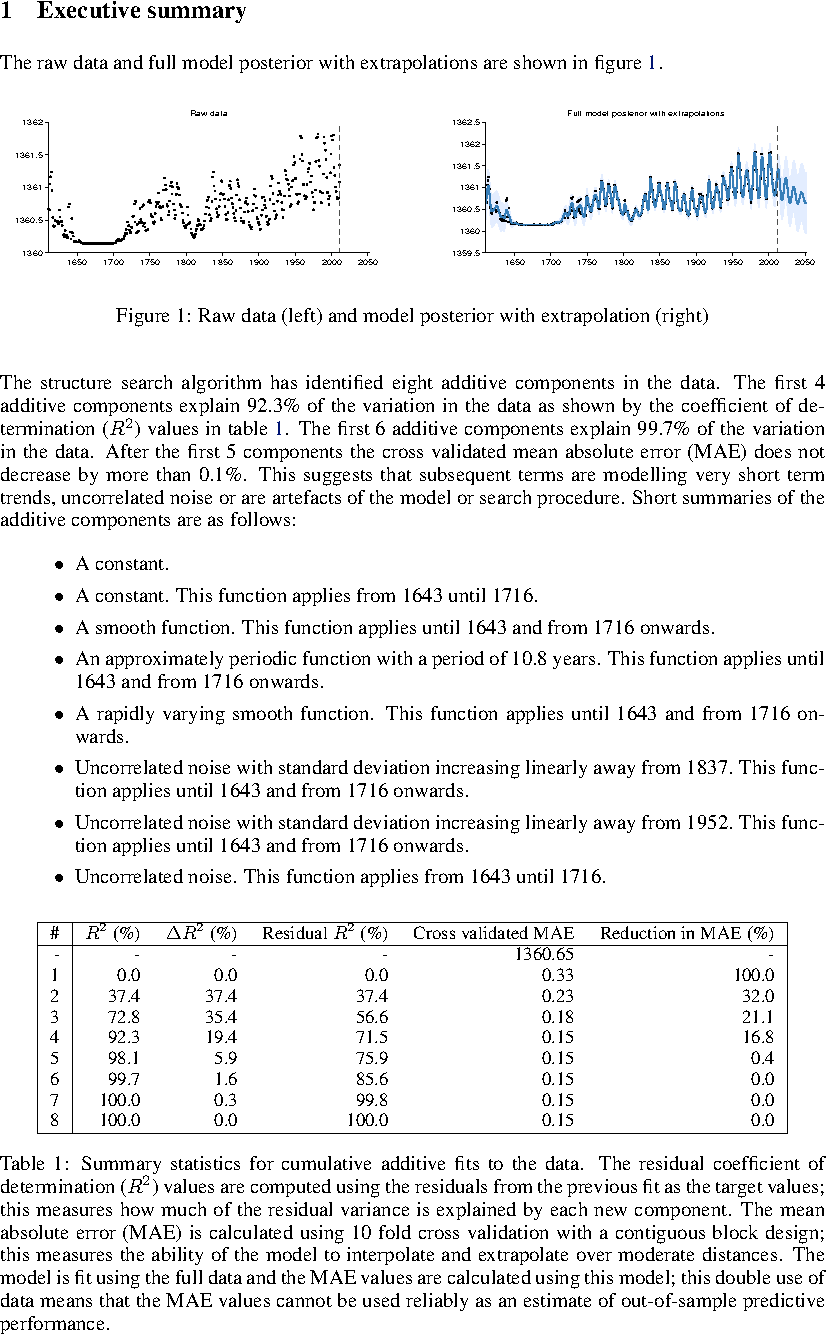
\includegraphics[trim=0.2cm 18.0cm 8cm 2cm, clip, width=0.98\columnwidth, height=0.45\columnwidth]{solarpages/pg_0002-crop}
\caption{
Solar irradiance data.}
\label{fig:solar}
\end{figure}

We show excerpts from the report automatically generated on annual solar irradiation data from 1610 to 2011 (figure~\ref{fig:solar}).
This time series has two pertinent features: a roughly 11-year cycle of solar activity, and a period lasting from 1645 to 1715 with much smaller variance than the rest of the dataset.
This flat region corresponds to the Maunder minimum, a period in which sunspots were extremely rare \citep{lean1995reconstruction}.
\procedurename{} clearly identifies these two features, as discussed below.

%After distributing and simplifying, the kernel corresponding to the first four components is as follows:
%\vspace{-0.5\baselineskip}
%\begin{itemize}
%  \itemsep0em
%  \item $\kC$
%  \item $\kCW(\emptyset,\kC)$
%  \item $\kCW(\kSE,\emptyset)$
%  \item $\kCW(\kSE \times \kPer,\emptyset).$
%\end{itemize}
%\vspace{-\baselineskip}
%$\kC + \kCW(\emptyset,\kC) + \kCW(\kSE,\emptyset) + \kCW(\kSE \times \kPer,\emptyset).$


\begin{figure}[h]
\centering
\fbox{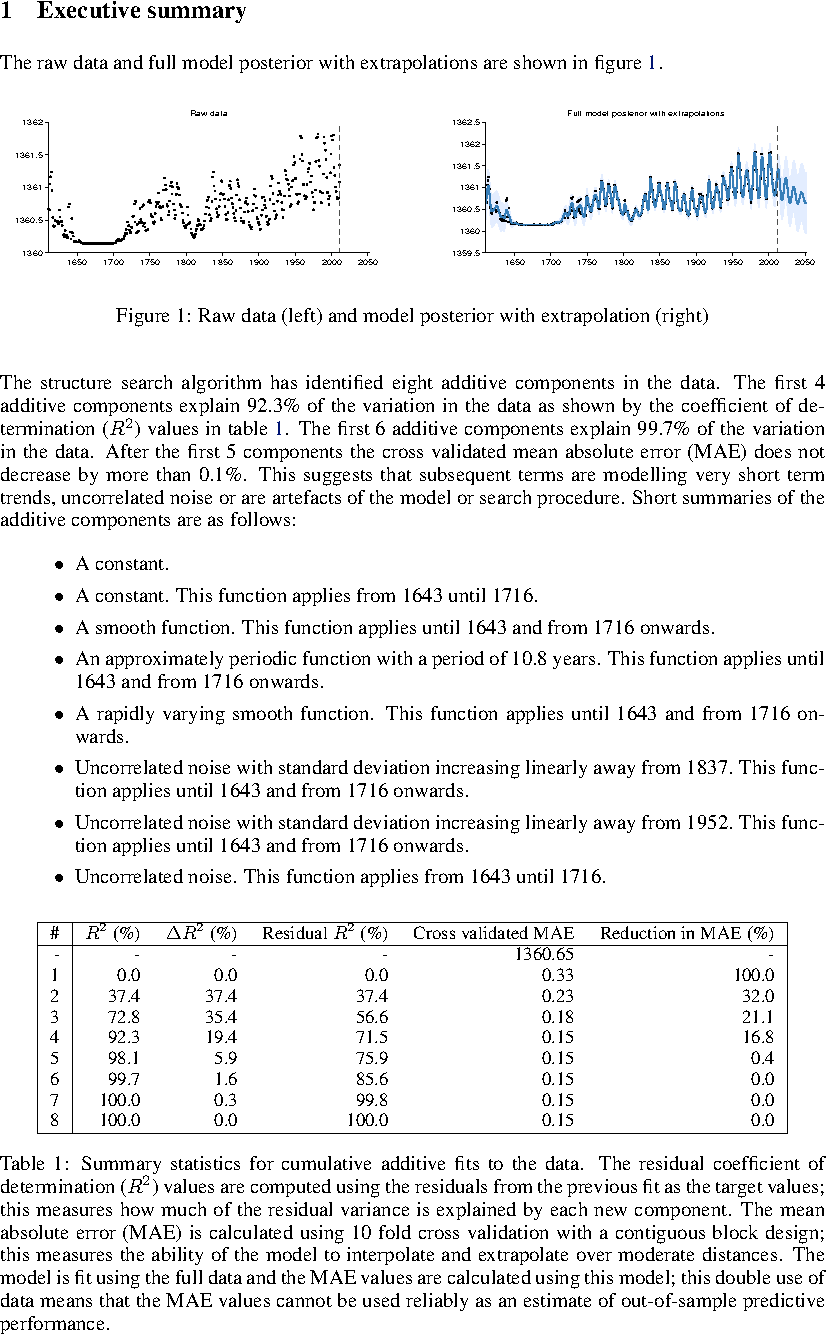
\includegraphics[trim=0cm 10.8cm 0cm 6.3cm, clip, width=0.98\columnwidth]{solarpages/pg_0002-crop}}
\caption{
Automatically generated descriptions of the components discovered by \procedurename{} on the solar irradiance data set.
The dataset has been decomposed into diverse structures with simple descriptions.}
\label{fig:exec}
\end{figure}
Figure \ref{fig:exec} shows the natural-language summaries of the top four components chosen by \procedurename{}.
%The short descriptions demonstrate how the kernel is split into univariate enveloping functions (from the change windows) and stationary kernels.
%
%
%The model uses 9 additive components to explain the data, and reports that the first 4 components explain more than 90\% of the variance in the data.
%This might seem incongruous with the observation that there are two main features of the data, but if we examine the first four components, we see that the first component is describing the mean of the dataset, the second is the Maunder minimum, the third describes the long-term trend, and the fourth describes the 11-year periodicity.
From these short summaries, we can see that our system has identified the Maunder minimum (second component) and 11-year solar cycle (fourth component).
These components are visualized in figures~\ref{fig:maunder} and \ref{fig:periodic}, respectively. 
%By examining the parameters of the kernels representing the solar cycle, \procedurename{} identified that the shape of the periodicity is near sinusoidal and also quantifies how quickly the exact shape of the sinusoid changes.
The third component corresponds to long-term trends, as visualized in figure~\ref{fig:smooth}.

\begin{figure}[ht]
\centering
\fbox{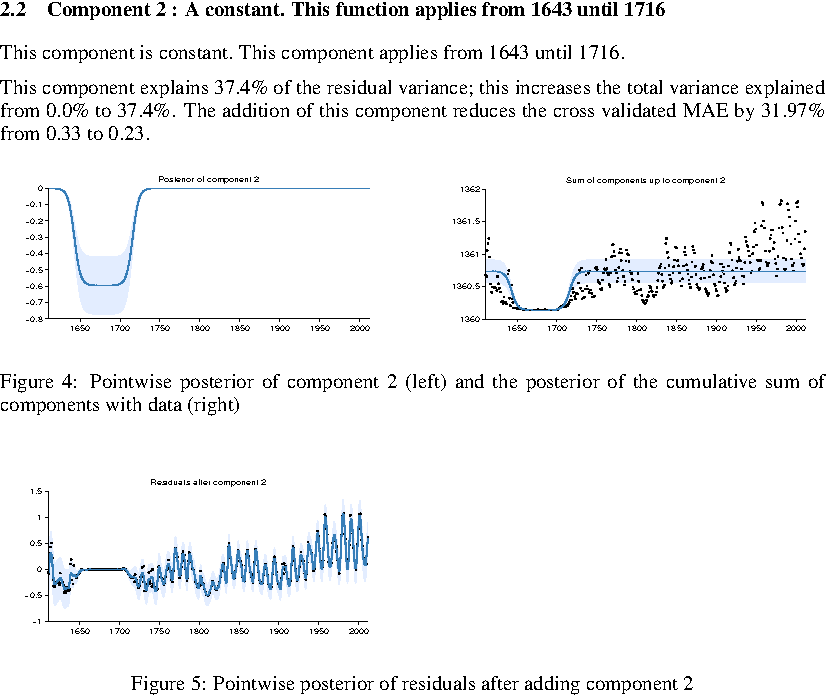
\includegraphics[trim=0cm 4.75cm 0cm 0.7cm, clip, width=0.98\columnwidth]{solarpages/pg_0005-crop}}
\caption{One of the learned components corresponds to the Maunder minimum.}
\label{fig:maunder}
\end{figure}

\begin{figure}[h!]
\centering
\fbox{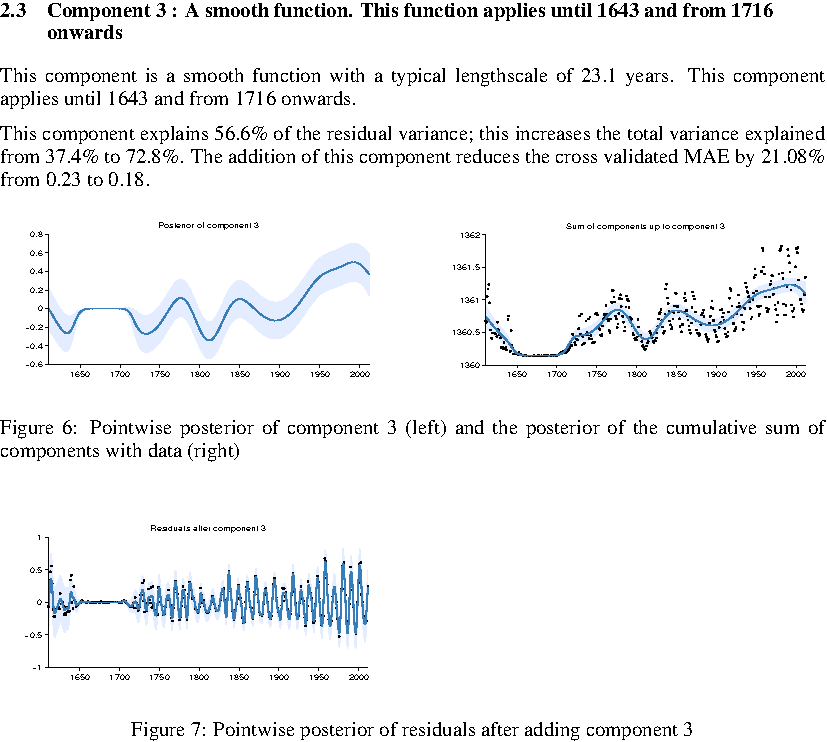
\includegraphics[trim=0cm 4.75cm 0cm 1cm, clip, width=0.98\columnwidth]{solarpages/pg_0006-crop}}
\caption{Characterizing the medium-term smoothness of solar activity levels.  By allowing other components to explain the periodicity, noise, and the Maunder minimum, \procedurename{} can isolate the part of the signal best explained by a slowly-varying trend.}
\label{fig:smooth}
\end{figure}

\subsection{Finding heteroscedasticity in air traffic data}
\label{sec:airline}

\begin{figure}[h]
\centering
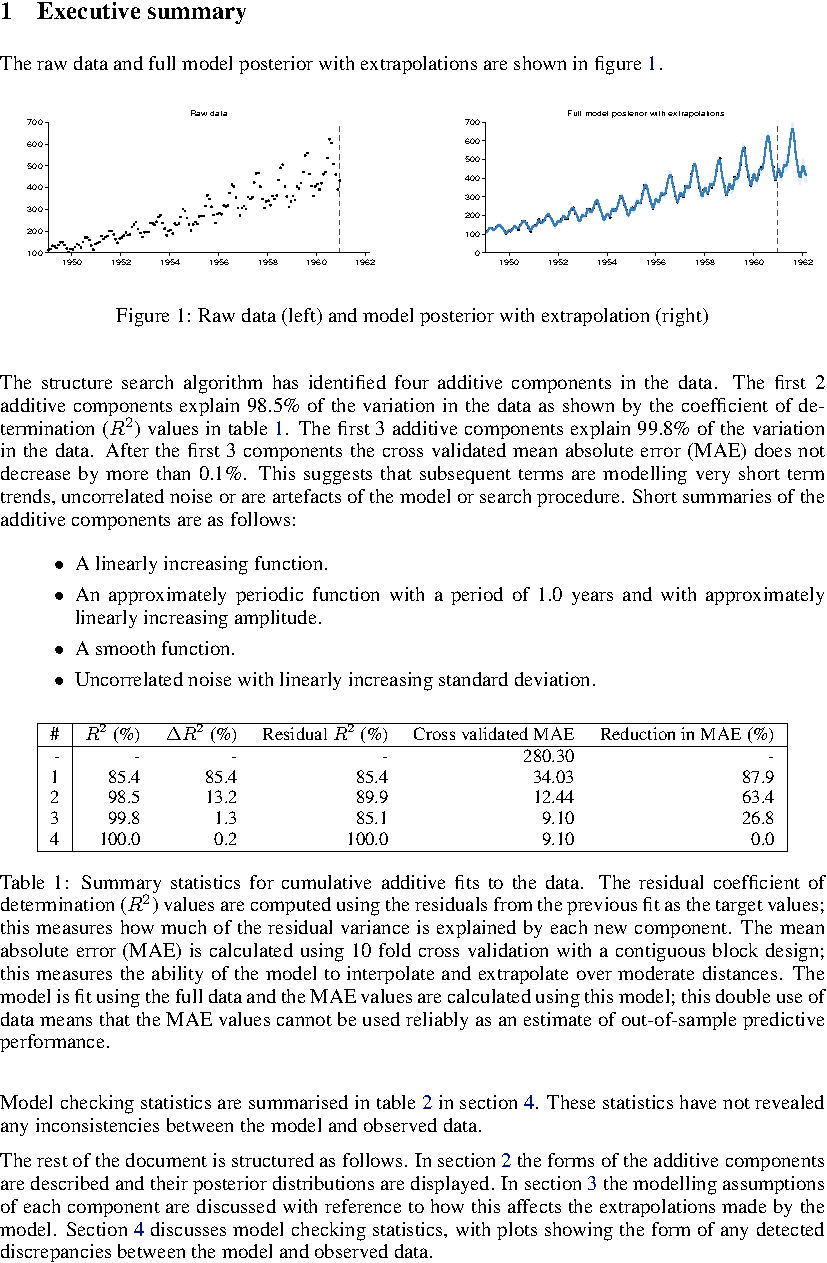
\includegraphics[trim=0.4cm 16.8cm 8cm 2cm, clip, width=0.98\columnwidth, height=0.45\columnwidth]{airlinepages/pg_0002-crop}
\caption{
International airline passenger monthly volume \citep[e.g.][]{box2013time}.}
\label{fig:airline}
\end{figure}

Next, we present the analysis generated by our procedure on international airline passenger data (figure~\ref{fig:airline}).
The model constructed by \procedurename{} has four components: $\kLin + \kSE \times \kPer \times \kLin + \kSE + \kWN \times \kLin$, with descriptions given in figure~\ref{fig:exec-airline}.

\begin{figure}[h]
\centering
\fbox{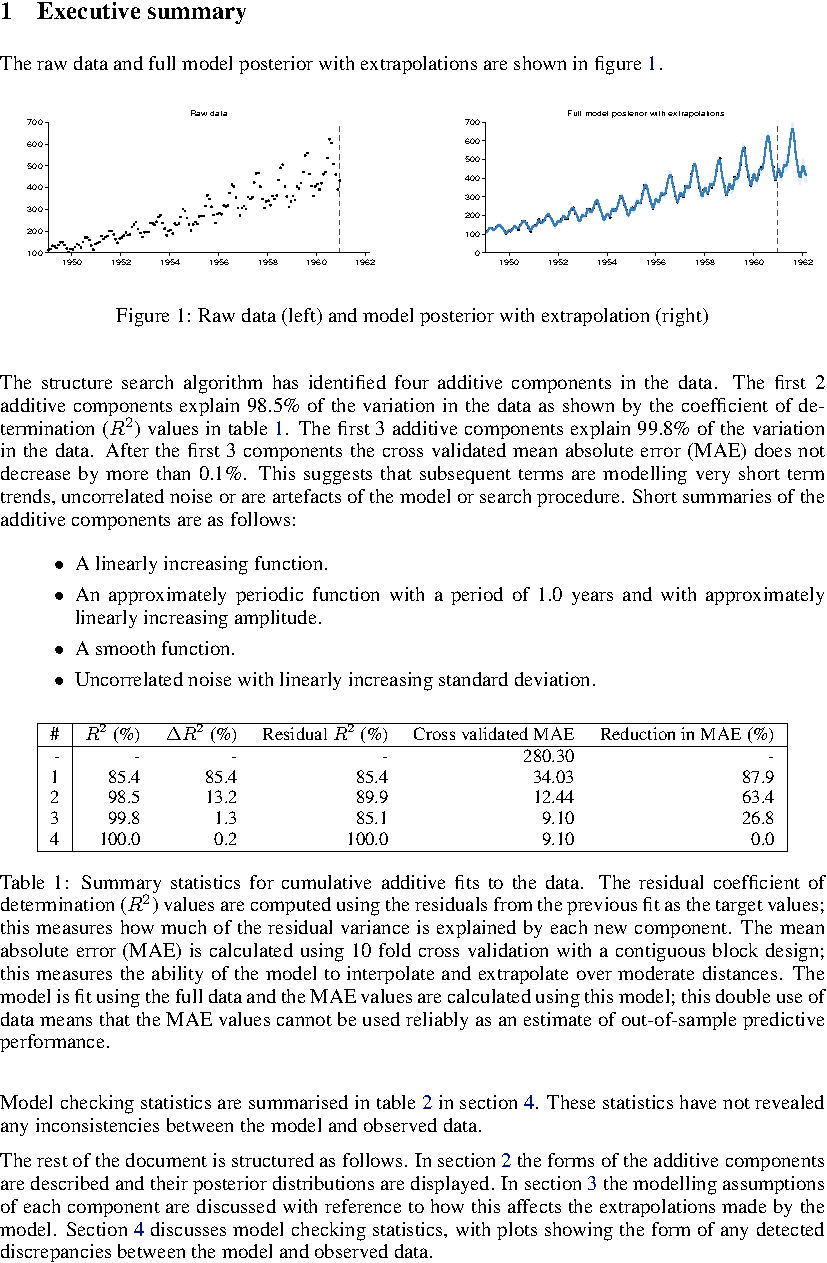
\includegraphics[trim=0cm 6.8cm 0cm 6cm, clip, width=0.98\columnwidth]{airlinepages/pg_0002-crop}}
\caption{
Short descriptions and summary statistics for the four components of the airline model.}
\label{fig:exec-airline}
\end{figure}

The second component (figure~\ref{fig:lin_periodic}) is accurately described as approximately ($\kSE$) periodic ($\kPer$) with linearly growing amplitude ($\kLin$).
%
\begin{figure}[h]
\centering
\fbox{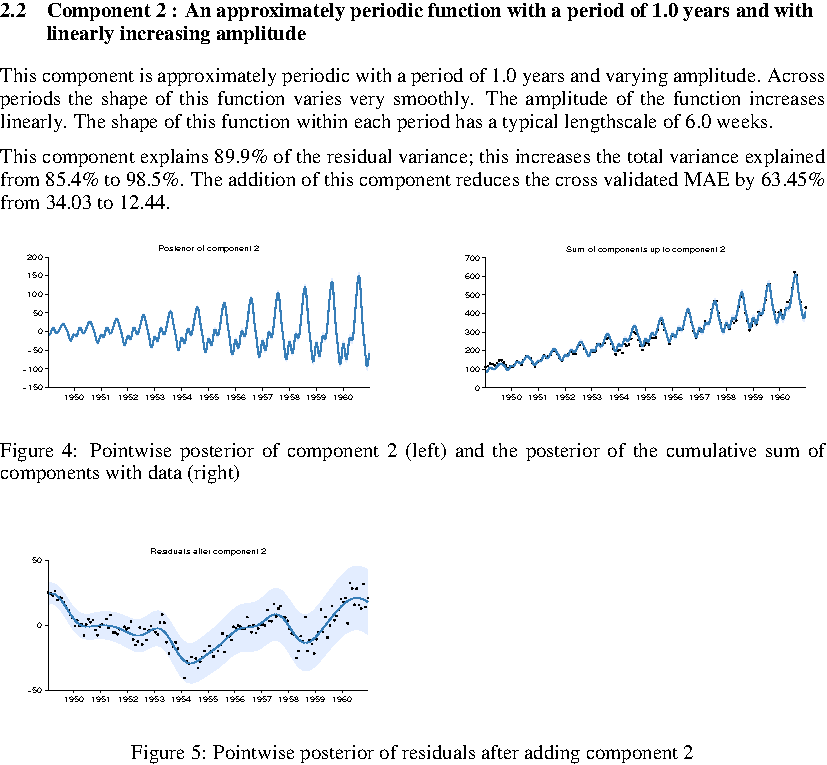
\includegraphics[trim=0cm 4.75cm 0cm 0cm, clip, width=0.98\columnwidth]{airlinepages/pg_0004-crop}}
\caption{Capturing non-stationary periodicity in the airline data}
\label{fig:lin_periodic}
\end{figure}
%
%\begin{figure}[h]
%\centering
%\fbox{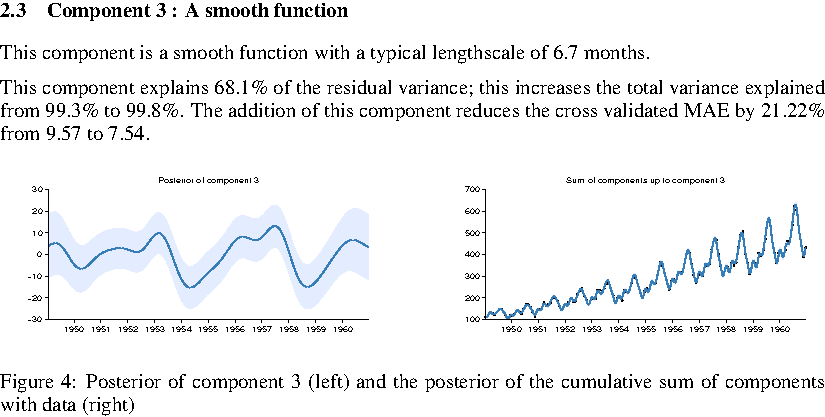
\includegraphics[trim=0cm 17cm 0cm 3.5cm, clip, width=0.98\columnwidth]{airlinepages/01-airline-separate-pages-5}}
%\caption{
%A caption.}
%\label{fig:exec}
%\end{figure}
%
%\paragraph{Linear heteroscedasticity}
%
By multiplying a white noise kernel by a linear kernel, the model is able to express heteroscedasticity (figure~\ref{fig:heteroscedastic}).
%
\begin{figure}[h]
\centering
\fbox{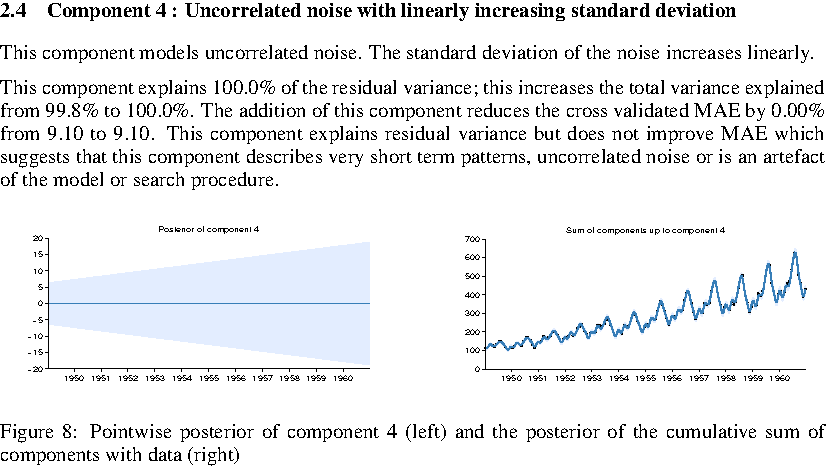
\includegraphics[trim=0cm 0cm 0cm 0cm, clip, width=0.98\columnwidth]{airlinepages/pg_0006-crop}}
\caption{Modeling heteroscedasticity}
\label{fig:heteroscedastic}
\end{figure}

\subsection{Comparison to equation learning}
\label{sec:eqn-learning-comp}

We now compare the descriptions generated by \procedurename{} to parametric functions produced by an equation learning system.
%We now compare the descriptions generated by \procedurename{} to those generated by Eureqa \citep{Eureqa}, an equation learning system.
%Eureqa \citep{Eureqa} is a system capable of producing parametric descriptions of time-series.
We show equations produced by Eureqa \citep{Eureqa} for the data sets shown above, using the default mean absolute error performance metric.
%\footnotetext{We experimented with the root mean squared error with Akaike information criterion penalisation (analogous to the criterion used by \procedurename{}) but occasionally observed severe overfitting.}


The learned function for the solar irradiance data is
\begin{align*}
\textrm{Irradiance($t$)} = 1361 + \alpha\sin(\beta + \gamma t)\sin(\delta + \epsilon t^2 - \zeta t)
\end{align*}
where $t$ is time and constants are replaced with symbols for brevity.
This equation captures the constant offset of the data, and models the long-term trend with a product of sinusoids, but fails to capture the solar cycle or the Maunder minimum.

The learned function for the airline passenger data is
\begin{align*}
\textrm{Passengers($t$)} = \alpha t + \beta\cos(\gamma - \delta t)\textrm{logistic}(\epsilon t - \zeta) - \eta
\end{align*}
which captures the approximately linear trend, and the periodic component with approximately linearly (logistic) increasing amplitude.
However, the annual cycle is heavily approximated by a sinusoid and the model does not capture heteroscedasticity.

\section{Related work}
\label{sec:related-work}

\paragraph{Building Structured Kernel Functions}
\cite{rasmussen38gaussian} devote 4 pages to manually constructing a composite kernel to model a time series of carbon dioxode concentrations.
In the supplementary material, we include a report automatically generated by \procedurename{} for this dataset; our procedure chose a model similar to the one they constructed by hand.
%A report automatically generated by \procedurename{} on this data set is included in the supplementary material and discovers a very similar model. 
Other examples of papers whose main contribution is to manually construct and fit a composite \gp{} kernel are \cite{klenske2012nonparametric} and \cite{lloydgefcom2012}.
\citet{diosan2007evolving, bing2010gp} and \citet{kronberger2013evolution} search over a similar space of models as \procedurename{} using genetic algorithms but do not interpret the resulting models.
Our procedure is based on the model construction method of \citet{DuvLloGroetal13} which automatically decomposed models but components were interpreted manually and the space of models searched over was smaller than that in this work. 

\paragraph{Equation learning}
\cite{todorovski1997declarative}, \cite{washio1999discovering} and \cite{schmidt2009distilling} learn parametric forms of functions specifying time series, or relations between quantities.
In contrast, \procedurename{} learns a parametric form for the covariance, allowing it to model functions without a simple parametric form.
%(We compare against an equation learning system in section~\ref{sec:eqn-learning-comp}.)
%Because our system specifies the more general\fTBD{JL: Sounds like we are claiming we are a super set of equation learning - we need more kernels to make this claim} covariance structure rather than the functions themselves, we are able to capture structure which does not have a simple parametric form.

\paragraph{Searching over open-ended model spaces}

This work was inspired by previous successes at searching over open-ended model spaces: matrix decompositions \citep{grosse2012exploiting} and graph structures \citep{kemp2008discovery}.
In both cases, the model spaces were defined compositionally through a handful of components and operators, and models were selected using criteria which trade off model complexity and goodness of fit.
Our work differs in that our procedure automatically interprets the chosen model, making the results accessible to non-experts.
%In another related paper, \cite{VikashScene13} automatically searches over models of 2D scenes.
%Automatic model search is possible whenever the following conditions are met: 1) we can define a large space of models by combining a small number of components in a small number of different ways; 2) inference can be performed for all models in this space; 3) a basic search procedure is sufficient to find accurate models.
%These conditions were also met for example in \citet{kemp2008discovery} who learned the structural form of a graph used to model human similarity judgments.  
%More generally, probabilistic programming [cite]\fTBD{Is there a canonical reference yet \eg I don't think there are any books} software automatically generates inference mechanisms for open-ended classes of models, enabling automatic model search.

%\fTBD{JL: Something about graphical models?}

%\NA{
%This is also true of - can we also cite some sort of graphical model work?
%}
%\fTBD{RG: Cite Kemp + Tenenbaum?}

%\paragraph{Standard inference methods}
%\fTBD{RG: How is this relevant?}
%The \procedurename language can express many regression motifs as \gp{}s for which inference is well understood.
%Probabilistic programming (cite) defines languages that describe generative models in such a way that %inference can be performed in each model.
%Extending the model search ideas in \procedurename to searches over probabilistic programs would be an interesting area for future research (cite Josh's workshop paper?).

\paragraph{Natural-language output}
To the best of our knowledge, our procedure is the first example of automatic description of nonparametric statistical models.
However, systems with natural language output have been built in the areas of video interpretation \citep{barbu2012video} and automated theorem proving \citep{GanesalingamG13}.

%\section{Numerical evaluation}
\section{Predictive Accuracy}
\label{sec:numerical}

\begin{figure*}[ht]
\centering
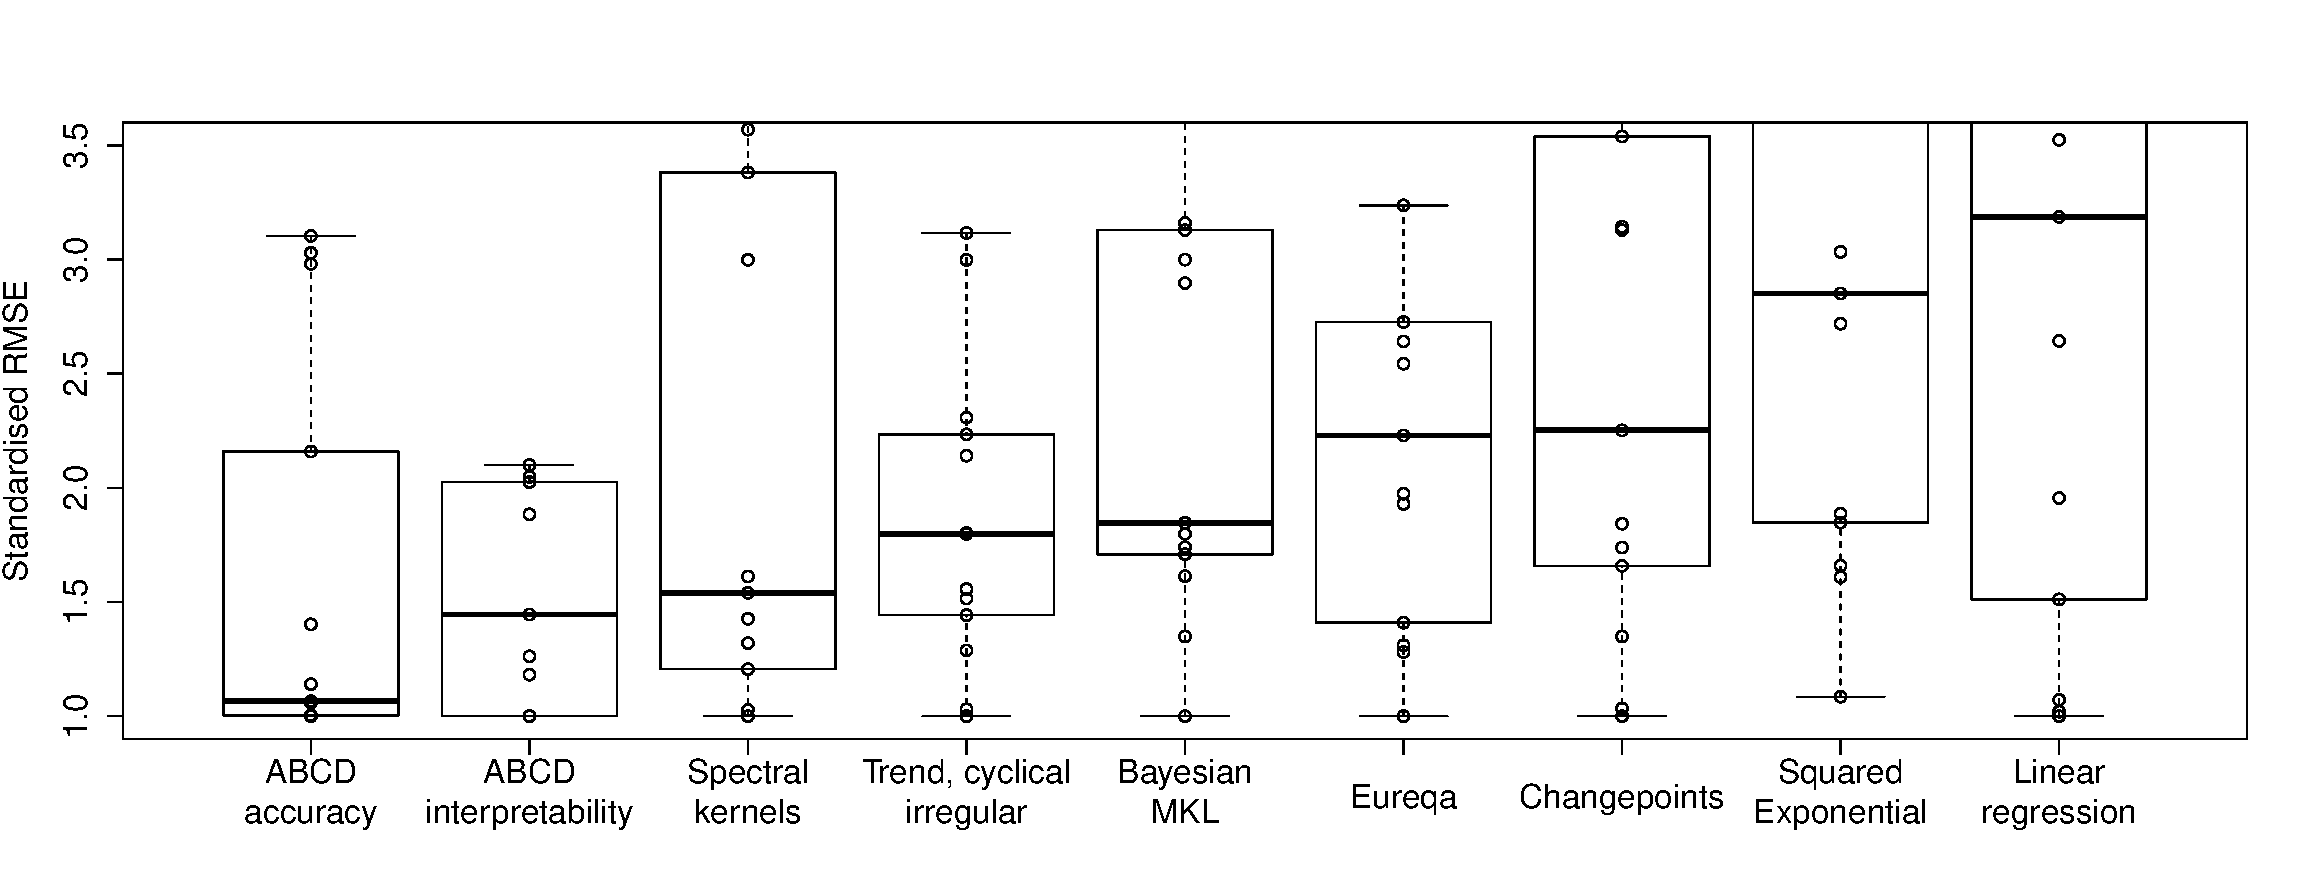
\includegraphics[width=\textwidth]{figures/box_extrap_wide}
\vspace{-0.8cm}
\caption{
Raw data, and box plot (showing median and quartiles) of standardised extrapolation RMSE (best performance = 1) on 13 time-series.
The methods are ordered by median.
}
\label{fig:box_extrap_dist}
\end{figure*}

In addition to our demonstration of the interpretability of \procedurename{}, we compared the predictive accuracy of various model-building algorithms at interpolating and extrapolating time-series.
\procedurename{} outperforms the other methods on average.% on average (\eg as measured by quantiles of performance metrics).
%\NA{However, the variability of the results suggests that there is room to improve the robustness of \procedurename.}
%\fTBD{JL: I'm trying to avoid claims of oversell - any thoughts on a measured statement?}

\paragraph{Data sets}

We evaluate the performance of the algorithms listed below on 13 real time-series from various domains from the time series data library \citep{TSDL}; plots of the data can be found at the beginning of the reports in the supplementary material.

\paragraph{Algorithms}

We compare \procedurename{} to equation learning using Eureqa \citep{Eureqa} and six other regression algorithms: linear regression, \gp{} regression with a single $\kSE$ kernel (squared exponential), a Bayesian variant of multiple kernel learning (MKL) \citep{bach2004multiple}, change point modeling
% / multi resolution Gaussian processes 
\citep{garnett2010sequential, FoxDunson:NIPS2012}, spectral kernels \citep{WilAda13} and trend-cyclical-irregular models \citep[e.g.][]{lind2006basic}.

% details of algorithms
We use the default mean absolute error criterion when using Eureqa.
All other algorithms can be expressed as restrictions of our modeling language (see table~\ref{table:motifs}) so we perform inference using the same search methodology and selection criterion\footnotemark~with appropriate restrictions to the language.
For MKL, trend-cyclical-irregular and spectral kernels, the greedy search procedure corresponds to a forward-selection algorithm. 
\footnotetext{We experimented with using unpenalised marginal likelihood as the search criterion but observed overfitting, as is to be expected.} 

We restricted to regression algorithms for comparability; this excludes models which regress on previous values of times series, such as autoregressive or moving-average models \citep[e.g.][]{box2013time}.
Constructing a language for this class of time-series model would be an interesting area for future research.

\paragraph{Interpretability versus accuracy}

BIC trades off model fit and complexity by penalizing the number of parameters in a kernel expression.
This can result in \procedurename{} favoring kernel expressions with nested products of sums, producing descriptions involving many additive components.
While these models have good predictive performance the large number of components can make them less interpretable.
We experimented with distributing all products over addition during the search, causing models with many additive components to be more heavily penalized by BIC.
We call this procedure \procedurename{}-interpretability, in contrast to the unrestricted version of the search, \procedurename{}-accuracy.

\paragraph{Extrapolation}

To test extrapolation we trained all algorithms on the first 90\% of the data, predicted the remaining 10\% and then computed the root mean squared error (RMSE).
The RMSEs are then standardised by dividing by the smallest RMSE for each data set so that the best performance on each data set will have a value of 1.

Figure~\ref{fig:box_extrap_dist} shows the standardised RMSEs across algorithms.
\procedurename{}-accuracy outperforms \procedurename{}-interpretability but both versions of have lower quartiles than all other methods.
%but the outliers of \procedurename{}, TCI and SP have similar values.

Overall, the model construction methods with greater capacity perform better: \procedurename{} outperforms trend-cyclical-irregular, which outperforms Bayesian MKL, which outperforms squared exponential.
Despite searching over a rich model class, Eureqa performs relatively poorly, since very few datasets are parsimoniously explained by a parametric equation.

Not shown on the plot are large outliers for spectral kernels, Eureqa, squared exponential and linear regression with values of 11, 493, 22 and 29 respectively.
All of these outliers occurred on a data set with a large discontinuity (see the call centre data in the supplementary material).
%All methods attempted to model this discontinuity using inappropriate components resulting in wild predictions.

%Also not shown on the plot is a very large outlier for EL of 493 (this was also on the call centre data).
%However, EL was the best performing algorithm on the wages dataset which shows an exponential increase after the industrial revolution.
%\procedurename can approximate an exponential function with a polynomial by combining $\kLin$ kernels but this is not a succinct expression in the current language.
%Expanding the modelling language of \procedurename is a natural area for future research.

%Somewhat surprisingly, TCI performs well despite its restrictive modelling assumptions (smooth functions and exact periodicity).
%Further inspection of the extrapolation has revealed that while TCI cannot model non-stationarity, its extrapolations of approximately periodic components can be quite effective.
%While \procedurename and SP will quickly become uncertain about a roughly periodic component, TCI will predict the average which is often more effective.
%This suggests that models composed of kernels of the form $(\kSE + \kC) \times \kPer$ will be effective for extrapolating approximately periodic components.

\paragraph{Interpolation}
To test the ability of the methods to interpolate, we randomly divided each data set into equal amounts of training data and testing data.
%We trained each algorithm on the training half of the data, produced predictions for the remaining half and then computed standardised RMSEs.
The results are similar to those for extrapolation and are included in the supplementary material.

\section{Conclusion}

Towards the goal of automating statistical modeling we have presented a system which constructs an appropriate model from an open-ended language and automatically generates detailed reports that describe patterns in the data captured by the model.
We have demonstrated that our procedure can discover and describe a variety of patterns on several time series.
%To the best of our knowledge this is the first system that can automatically describe any model in an open-ended class of nonparametric models in natural language.
Our procedure's extrapolation and interpolation performance on time-series are state-of-the-art compared to existing model construction techniques.
We believe this procedure has the potential to make powerful statistical model-building techniques accessible to non-experts.

%Thinking towards extending this line of work many questions and challenges are raised which we briefly outline.

%\paragraph{Accuracy versus interpretability}
% DD: we already talk about this in the experimental section
%Typical machine learning research focuses on predictive performance rather than interpretability, likely due to the difficulty of assessing the interpretability of a method in an objective manner.
%Requiring that statistical models can be automatically described constrains the models that can be used over and above the traditional constraints of tractability.

%\paragraph{A sufficiently large class of models}
%To be non-trivial.

%\paragraph{Computational complexity}
%\fTBD{JL,DD: This can potentially be shortened - or even removed}
%\fTBD{JL: At the least it should not be a verbatim quote of JBT}
%\procedurename{} is embarassingly parallel, and can be run overnight on a cluster.
%This is computationally expensive compared to fitting only one or a small number of models.
%However, this computational cost may be reasonable when compared to the cost of having a human researcher iteratively propose, fit, and refine a series of models, especially when one considers the size and scope of the space of models that is searched, and the fact that all steps of model construction, evaluation and search are automatic.

%In our experience, working statisticians, machine learners, and data scientists rarely if ever explore such a space so systematically, partly because of the cost in terms of both their own time and computation time.
%The artificial intellgience presented in this paper is still quite primitive and naive, and the space of models we can consider automatically is still quite limited compared to what humans can do.
%However, in evaluating the limitations of these methods, and prospects for future work of this sort, other factors might loom larger than computational efficiency.



%\paragraph{Automatic description of methods}



%\paragraph{When is a description of a model useful as a description of data?}

%\fTBD{Shorten me significantly}

%\procedurename produces models, $M$, of the form $f = \sum_i f_i$ where $f_i \dist \gp{}(0, \kernel_i)$.
%The form of $M$ is chosen to be that which best explains observations of $f$, denoted by $D$, as measured by approximate marginal likelihood.

%In the reports generated by \procedurename, we show plots of the posterior $p(f_i^*\given M,D)$ but the natural-language descriptions are of typical elements of the prior $p(f_i^*\given M)$ given the fitted model \ie they are descriptions of the model rather than descriptions of the data.

%Despite fitting the model to the data by maximising the marginal likelihood $p(D\given M)$ the selected model may be a poor description of the data if the data contains features not easily expressed by the language of models defined by \procedurename.
%To test for when this is the case we have begun experimenting with posterior predictive checks to assess the models produced by \procedurename following the techniques of \cite{Gelman1996} (see reports in the supplementary material).
%In fact, the posterior predictive checks take the form of comparing the expectation of statistics under the prior and posterior of each component \ie they are testing whether or not typical elements of the posterior $p(f_i^*\given M,D)$ are typical elements of $p(f_i^*\given M)$.

%However, model checking for Gaussian processes, even those with simple kernels, is under-researched so we leave their description and more detailed analysis for future work. 

%\paragraph{Other systems}
%The system presented in this paper is just one example of a system combining these elements, for performing supervised regression.
%\citep{grosse2012exploiting} provides an earlier example with builds unsupervised models.
%Similar systems could be constructed in other learning scenarios, such as sequence modeling or semi-supervised learning.

\paragraph{Source Code}
Source code to perform all experiments will be available on github upon publication.
%\href{http://www.github.com/jamesrobertlloyd/gpss-research}
%{\texttt{github.com/jamesrobertlloyd/gpss-research}}}
%All \gp{} hyperparameter tuning was performed by automated calls to the GPML toolbox\footnote{Available at 
%\href{http://www.gaussianprocess.org/gpml/code/}
%{\texttt{www.gaussianprocess.org/gpml/code/}}
%}

%\section{Discussion}

%\begin{quotation}
%``The availability of 'user-friendly' statistical software has caused authors to become increasingly careless about the logic of interpreting their results, and to rely uncritically on computer output, often using the 'default option' when something a little different (usually, but not always, a little more complicated) is correct, or at least more appropriate.''
% In trying to practice this art, the Bayesian has the advantage because his formal apparatus already developed gives him a clearer picture of what to expect, and therefore a sharper perception for recognizing the unexpected.

%\defcitealias{dyke1997avoid}{G. Dyke, 1997}
%\hspace*{\fill}\citet{Jaynes85highlyinformative}
%\hspace*{\fill}\citetalias{dyke1997avoid}
%\end{quotation}

%In this paper, we exhibited the output of a method for automatically constructing and summarizing a compositional Gaussian process regression model in natural language.
%These summaries can enable human experts and non-experts to understand the implications of a model, check its plausibility, and notice structure not yet captured by the model.

\bibliography{gpss}
\bibliographystyle{format/icml2014}

\end{document} 
